%Reporte sobre la actividad del producto 4
\documentclass[notitlepage,12pt]{article}

%El documento estara en español, usar paquete en español
\usepackage[spanish]{babel}
\selectlanguage{spanish}
\usepackage[utf8]{inputenc}
%Permite colores
%Permite incorporar imagenes
\usepackage{graphicx}
\usepackage{color}
%Escribir formulas matematicas
\usepackage{amsmath}
%topmatter (titulo, autor, fecha)
\title{Aproximaci\'on mediante polinomios de Taylor}
\author{Hugo de Jes\'us Valenzuela Chaparro}
\date{\today}

\begin{document}
\maketitle

\section{Polinomio de Taylor}
Los valores de funciones polinomiales pueden determinarse efectuando un n\'umero finito de adiciones y multiplicaciones, no obstante,
otras funciones, entre ellas las logar\'itmicas, exponenciales y trigonom\'etricas, no pueden evaluarse tan f\'acilmente. Muchas
funciones pueden aproximarse usando polinomios, uno de los m\'as utilizados es la f\'ormula de Taylor. La cual se establece as\'i:

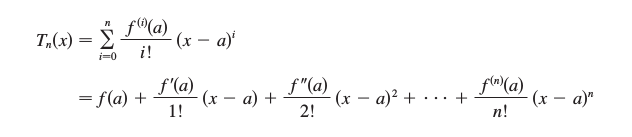
\includegraphics[scale=0.5]{ptaylor}

La cual sirve para aproximar la funci\'on f(x). Se le conoce como polinomio de Taylor de grado n, centrado en a. En particular, si a=0 
entonces es conocido como polinomio de Maclaurin.

\section{Aproximaciones}

\subsection{$sin(x)$}
Se aproxim\'o con polinomios de Maclaurin de grado 1, 3, 5 y 7.

C\'ODIGO DE MAXIMA:
\begin{verbatim}
f(x):= sin(x);
P1(x):=taylor(f(x), x, 0, 1);
P3(x):=taylor(f(x), x, 0, 3);
P5(x):=taylor(f(x), x, 0, 5);
P7(x):=taylor(f(x), x, 0, 7);
fortran(P1(x));
fortran(P3(x));
fortran(P5(x));
fortran(P7(x));
tex(P1(x));
tex(P3(x));
tex(P5(x));
tex(P7(x));
plot2d ([f(x),P1(x),P3(x),P5(x),P7(x)], [x, -%pi, %pi],
[color, red, blue, black, magenta, green],
[legend, "y=sin(x)", "y=P1(x)", "y=P3(x)", "y=P5(x)", "y=P7(x)"],
[axes,true], [xlabel,"X"] , [ylabel,"Y"]);
\end{verbatim}
Gr\'afica:


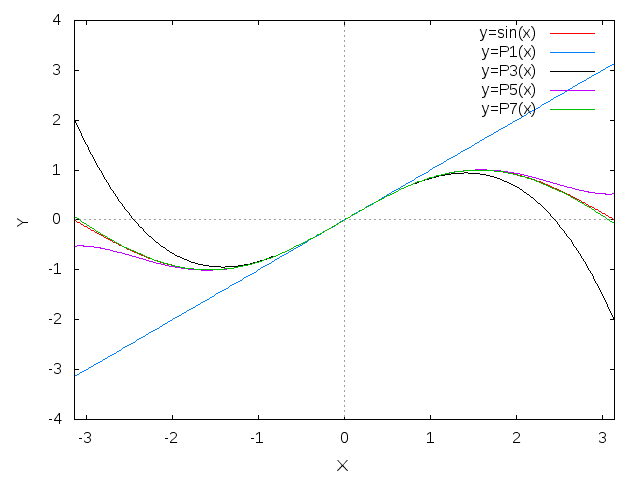
\includegraphics[scale=0.5]{sinx_ptaylor}

\subsection{$log(1+x)$}
Se aproxim\'o con polinomios de Maclaurin de grado 4, 7, 11 y 16.

C\'ODIGO DE MAXIMA:
\begin{verbatim}
f(x):= log(1+x);
P4(x):=taylor(f(x), x, 0, 4);
P7(x):=taylor(f(x), x, 0, 7);
P11(x):=taylor(f(x), x, 0, 11);
P16(x):=taylor(f(x), x, 0, 16);
fortran(P4(x));
fortran(P7(x));
fortran(P11(x));
fortran(P16(x));
tex(P4(x));
tex(P7(x));
tex(P11(x));
tex(P16(x));
plot2d ([P4(x),P7(x),P11(x),P16(x),f(x)], [x, -2, 2], [y, -4, 4],
[color, green, blue, black, magenta, red],
[legend, "T4", "T7", "T11", "T16", "Log(1+x)"],
[axes,true], [xlabel,"X"] , [ylabel,"Y"]);
\end{verbatim}
Gr\'afica:


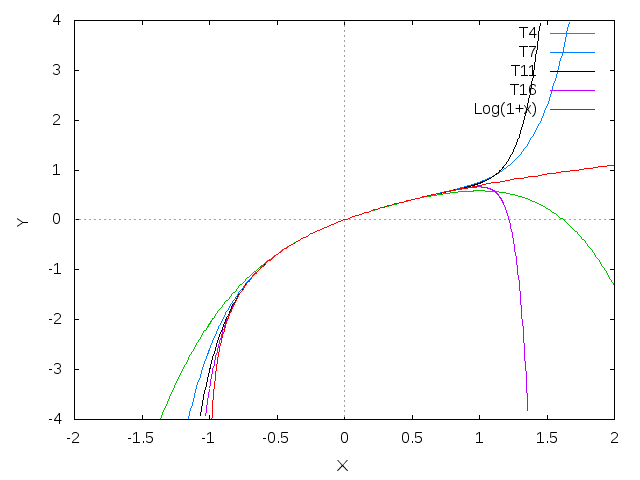
\includegraphics[scale=0.5]{log(1+x)_ptaylor}

\subsection{$log(cos(x))$}
Se aproxim\'o con polinomios de Maclaurin de grado 4, 7, 9 y 14.

C\'ODIGO DE MAXIMA:
\begin{verbatim}
f(x):= log(cos(x));
P4(x):=taylor(f(x), x, 0, 4);
P7(x):=taylor(f(x), x, 0, 7);
P9(x):=taylor(f(x), x, 0, 9);
P14(x):=taylor(f(x), x, 0, 14);
fortran(P4(x));
fortran(P7(x));
fortran(P9(x));
fortran(P14(x));
tex(P4(x));
tex(P7(x));
tex(P9(x));
tex(P14(x));
plot2d ([P4(x),P7(x),P9(x),P14(x),f(x)], [x, -%pi/2, %pi/2], [y, -4, 4],
[color, green, blue, black, magenta, red],
[legend, "T4", "T7", "T9", "T14", "Log(cos(x))"],
[axes,true], [xlabel,"X"] , [ylabel,"Y"]);
\end{verbatim}
Gr\'afica:


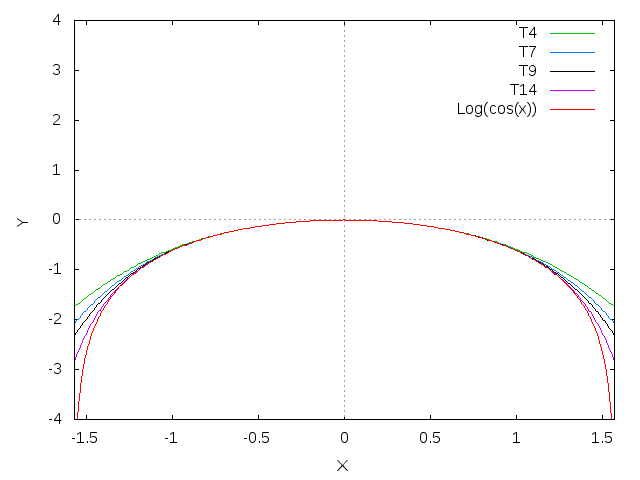
\includegraphics[scale=0.5]{log(cosx)_ptaylor}

\subsection{$e^x/cos(x)$}
Se aproxim\'o con polinomios de Maclaurin de grado 4, 7, 9 y 14.

C\'ODIGO DE MAXIMA:
\begin{verbatim}
f(x):=exp(x)/cos(x);
P4(x):=taylor(f(x), x, 0, 4);
P7(x):=taylor(f(x), x, 0, 7);
P9(x):=taylor(f(x), x, 0, 9);
P14(x):=taylor(f(x), x, 0, 14);
fortran(P4(x));
fortran(P7(x));
fortran(P9(x));
fortran(P14(x));
tex(P4(x));
tex(P7(x));
tex(P9(x));
tex(P14(x));
plot2d ([P4(x),P7(x),P9(x),P14(x),f(x)], [x, -4, 4], [y, -8, 8],
[color, green, blue, black, magenta, red],
[legend, "T4", "T7", "T9", "T14", "exp(x)/cos(x)"],
[axes,true], [xlabel,"X"] , [ylabel,"Y"]);
\end{verbatim}
Gr\'afica:


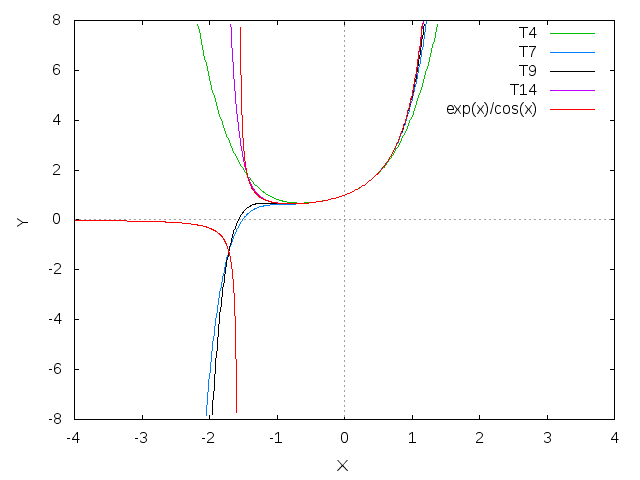
\includegraphics[scale=0.5]{exp(x)_cos(x)_ptaylor}

\subsection{$(1+x)e^x$}
Se aproxim\'o con polinomios de Maclaurin de grado 4, 7, 9 y 14.

C\'ODIGO DE MAXIMA:
\begin{verbatim}
f(x):=(1+x)*exp(x);
P4(x):=taylor(f(x), x, 0, 4);
P7(x):=taylor(f(x), x, 0, 7);
P9(x):=taylor(f(x), x, 0, 9);
P14(x):=taylor(f(x), x, 0, 14);
fortran(P4(x));
fortran(P7(x));
fortran(P9(x));
fortran(P14(x));
tex(P4(x));
tex(P7(x));
tex(P9(x));
tex(P14(x));
plot2d ([P4(x),P7(x),P9(x),P14(x),f(x)], [x, -8, 8], [y, -8, 8],
[color, green, blue, black, magenta, red],
[legend, "T4", "T7", "T9", "T14", "(1+x)*exp(x)"],
[axes,true], [xlabel,"X"] , [ylabel,"Y"]);
\end{verbatim}
Gr\'afica:


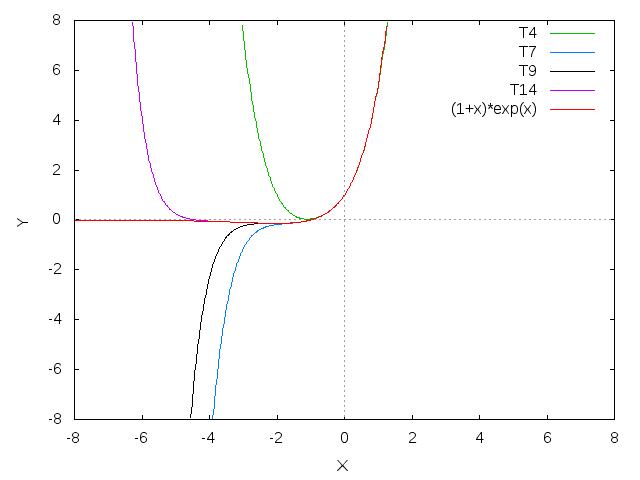
\includegraphics[scale=0.5]{(1+x)(exp(x))}











\end{document}
